\documentclass[letterpaper, onecolumn,10pt]{IEEEtran}

\usepackage{graphicx}
\usepackage{amssymb}
\usepackage{amsmath}
\usepackage{amsthm}

\usepackage{alltt}
\usepackage{float}
\usepackage{color}
\usepackage{url}
\usepackage{listings}
\usepackage{ifthen}
\usepackage{relsize}


\usepackage[TABBOTCAP, tight]{}

\usepackage{geometry}
\geometry{textheight=8.5in, textwidth=6in}

%random comment

\newcommand{\cred}[1]{{\color{red}#1}}
\newcommand{\cblue}[1]{{\color{blue}#1}}

\usepackage{hyperref}
\usepackage{geometry}
\usepackage{caption}
\usepackage{url}
\usepackage{natbib}

\begin{document}
    \begin{titlepage}
    \newcommand{\HRule}{\rule{\linewidth}{0.5mm}}
    \center
    \textsc{\Large Oregon State University}\\[1.5cm]
    \textsc{\Large ST 314}\\[0.5cm]
    \textsc{\Large Summer 2019}\\[0.5cm]
    \HRule \\[0.4cm]
    { \huge \bfseries Data Analysis One}\\[0.4cm] % Title of your document
    \HRule \\[1.5cm]
    \begin{minipage}{0.4\textwidth}
        \begin{flushleft} \large
        \emph{Author:}\\
        Thomas Noelcke
        \end{flushleft}
    \end{minipage}
    \begin{minipage}{0.4\textwidth}
        \begin{flushright} \large
        \emph{Instructor:} \\
        Katie Jager\\
        \end{flushright}
    \end{minipage}\\[2cm]
		\end{titlepage}
        
        \iffalse
        For each random variable:
        a. State the distribution that will best model random variable. Choose from the common distributions:
        Uniform, Exponential or Normal distribution. Explain your reasoning.
        b. State the parameter values that describe the distribution.
        c. Give the probability density function. 

        Random Variable 1.
        The maintenance manager at a chemical facility know that times between repairs for a specific chemical
        reactor is modeled by a distribution that is positively skewed, with no upper limit. The average time
        between a repair is 100 days.
        Random Variable 2.
        An agricultural study found the percent of butterfat in the milk of 2-year old Canadian dairy cows is
        symmetrically distributed. The percent of butterfat in the study had an average of 4.5\% and a standard
        deviation of 0.4\%. The butterfat percentages were more likely to be near the mean than further away.
        Random Variable 3.
        During a routine check, an engineer discovers that a pump has failed for a production process between the time period of 2:00PM and 4:00PM. Consider the time of failure is a random variable, where the pump has an equal chance of failing at anytime during the period between 2:00PM and 4:00PM
        \fi
		\section{Part 1}
		    \subsection{Random Variable 1}
		        This variable would be best modeled by the exponential distribution. This is because it has no upper limit and is positively skewed. Additionally, we know the average but not the standard distribution. To best model this distribution we only need one parameter, the average. Given the average we can calculate the value for lambda. Show below is the probability density function.
		        \[
		        f_x =
		        \begin{cases}
		            \frac{1}{100}e^{-\frac{1}{100}x} &\  x \geq 0\\
		            0 &\ x < 0\\
		        \end{cases}
		        \]\\
                    		        
		        
            \subsection{Random Variable 2}
                This random variable would be best modeled by the normal distribution. The probability is symmetrical where it is more likely that the values are closer to the mean. The distribution of the dairy cows also has a calculated standard deviation which makes it easy to model with the normal distribution. For this distribution we need the average value for the distribution in question and the standard distribution. In this case the average is 4.5\% and the standard deviation is 0.4\%. Shown below is the probability density function.\\
                
                \[
                    f_x = \frac{1}{\sqrt{2\pi0.4^{2}}}\Big{e}^-\frac{(x - 4.5)^{2}}{0.8^{2}}
                \]
                
            \subsection{Random Variable 3}
                This random variable would be best modeled by the Uniform distribution. This is because between 2pm and 4pm the pump was in a failure state. This distribution also works well because there are clear upper and lower bounds to the distribution and a single value during that period of time. In this cause we only need the upper and lower bounds for the distribution and the value for the distribution. In this case the upper and lower bounds are 2 to 4. We will let the chance of failure at any given one point during the the two hours be represented by the value 1/120. Below is the the probability density function.\\
                
                \[
                    f_x =
                    \begin{cases}
                        \frac{1}{120} &\  2 \geq x \leq 4\\
                        0 &\ x > 2, x < 4 
                    \end{cases}
                \]
                
                
                
        \iffalse
        Part 2. (9 points) Normal Distributions
        The distribution represents the approximate distribution of
        entry-level salaries for Mechanical Engineers in the US
        according to Glassdoor.com. Use this distribution to answer
        the following questions. Show work or R code for each.
        a. (2 points) State the average and standard deviation values
        for the salary distribution.
        b. (2 points) Suppose an engineer claims their salary is
        \$59000/year, how many standard deviations away from
        the mean is their salary? (Hint: This is the z score)
        c. (2.5 points) According to this distribution, what is the
        probability a mechanical engineer’s salary is below
        \$59000?
        d. (2.5 points) What salary amount represents the 85th
        percentile? 
        \fi
        \section{Part 2}
            \subsection{}
                The average appears to be 75,000\$ according to the distribution shown in the picture. based on the 65, 95 99 rule I would estimate that the standard deviation appears to be x. I've placed some R code and a recreation of the plot which I've used for the rest of the calculations below.\\
                
                \begin{lstlisting}[language=R]
                    salary = function(x) {dnorm(x, mean = 75, sd=10)+75}
                    r = seq(40, 110, 0.1)
                    lab = seq(45, 105, 10)
                    plot(r, salary(r), xlab="", main="Salary", lwd = 2, xaxt="n")
                    axis(1, at = lab, las=2)
                \end{lstlisting}
                
                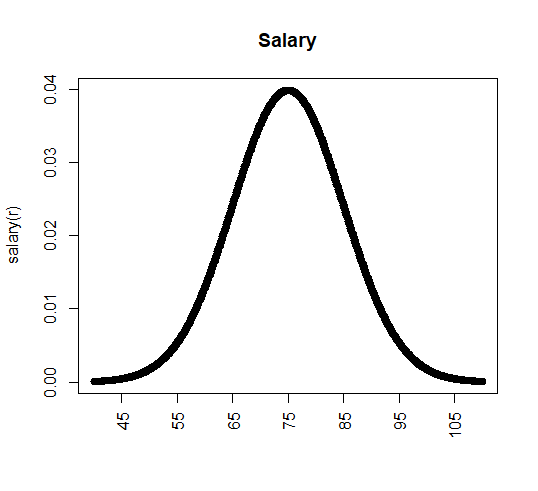
\includegraphics{week2/plot.png}
                
            \subsection{}
                For this problem we can simply calculate a Z Score and determine how far away that 59,000\$ is away from the mean.\\
                
                \[
                    Z = \frac{x - \mu}{\sigma}\\
                \]
                \[
                    Z = \frac{59000 - 75000}{10000} = -1.6\\
                \]
                
                The salary of 59,000\$ per year is 1.6 standard deviations less than the mean.\\
                
            \subsection{}
                To find the probability that an engineers salary is less than 59000 I used R. I've included the R code that I used to find the answer below as well as the output to the console.
                
                \begin{lstlisting}[language=R]
                    salaryProp = function(x) {pnorm(x, mean = 75, sd = 10)}
                    salaryProp(59)
                \end{lstlisting}
                
                \begin{lstlisting}[language=sh]
                    > salaryProp = function(x) {pnorm(x, mean = 75, sd = 10)}
                    > salaryProp(59)
                    [1] 0.05479929
                \end{lstlisting}
                
            \subsection{}
                To find the 85th percentile of mechanical engineers salary I decided to user R. I've include the R code that i used to find the answer below as well as the output from the console.
                
                \begin{lstlisting}[language=R]
                    salary = function(x) {qnorm(x, mean = 75, sd=10)}
                    salary(0.85)
                \end{lstlisting}
                
                \begin{lstlisting}[language=sh]
                    > salary = function(x) {qnorm(x, mean = 75, sd=10)}
                    > salary(0.85)
                    [1] 85.36433
                \end{lstlisting}
                This means that the salary that is at the 85th precentile is 85,363.33\$.\\
        \iffalse
Part 3. (12 points) Simulation of Gamma Random Variables
Background: When we use the probability density function to find probabilities for a random variable, we are
using the density function as a model. This is a smooth curve, based on the shape of observed outcomes for the
random variable. The observed distribution will be rough and may not follow the model exactly. The probability
density curve, or function, is still just a model for what is actually happening with the random variable. In other
words, there can be some discrepancies between the actual proportion of values above x and the proportion of
area under the curve above the same value x. Our expectation is as the number of observations increase, literally
or theoretically, the observed distribution will align more with the density curve. Over the long run, the differences
are negligible, the model is sufficient and more convenient to find desired information. 
Intellectual Property of Katie Jager ©
3
Simulation: Use R to simulate 1000 observations from a gamma distribution. To begin alpha = 2 and beta = 7.
Highlight and run the parameters and observation values. Run the simulation code to plot the observations and fit
the probability density function over the observations. You don’t need to change anything. You may run the
section all at once by highlighting all of the section and running it by clicking the run button at the top of the
script window.
a. Given the values are from a gamma distribution with alpha = 2 and beta = 7,
i. (1 point) What is the expression for the probability density function?
ii. (2 points) What is the average and standard deviation of random variable? Show work.
iii. (2 points) What is the probability x is less than 4? Show work.
b. (1 point) Run the simulation and paste your plot. Comment on the general shape of the distribution. How well
does the density curve fit the observations?
c. (1 point)What is the exact proportion of values below 4? How does the actual proportion compare to the
probability from the density curve in part 2-a-iii?
d. (1 point) Increase the number of observation to 10000, rerun the simulation. Paste your plot. How does
increasing the number of observations affect the fit of the density curve?
e. (1 point) What is the exact proportion of values below 4? How does increasing the number of observations
affect the accuracy of the model? Make a comparison between this proportion and 2-a-iii and 2c.
f. (1 point) Rerun the simulation with alpha = 1, beta = 7, and observations = 10000. Paste your plot. Comment
on the general shape of the distribution.
g. (2 points) This model is a special case of the gamma distribution, what is it specifically? What is the expression
for the probability density function?
h. Optional: Change the parameter values and take note of the effect of increasing or decreasing parameter
values. 
        \fi

        \section{Part 3}
            \subsection{}
                \paragraph{i}
                    The expression of the probability density function is shown below:
                    
                    \[
                        \mathlarger{
                        f_x =
                        \begin{cases}
                            \frac{1}{7^{\alpha}\gamma(2)}xe^{\frac{-x}{7}} &\ x \geq 0\\
                            0 &\ otherwise\\
                        \end{cases}
                        }
                    \]
                \
            
		        \paragraph{ii}
		            The average and standard deviation are shown below.
		            Average Expected Value:
		            \[E(x) = u_x = \alpha\Beta\]
		            \[E(x) = 14\]
		            
		            Standard Deviation:
		            
		            \[V(x) = \sigma_x^{2} = \alpha\Beta^{2}\]
		            \[sd = sqrt{2*7^2)}\]
		            \[sd = 9.8994\]
		            
		        \paragraph{iii}
		            I chose to use R for this problem below is the r code I used as well as the results from the terminal.
		        \begin{lstlisting}[language=R]
                    gamma = function(x) {pgamma(x,2, (1/7))}
                    gamma(4)
                \end{lstlisting}
                
                \begin{lstlisting}[language=sh]
                    > gamma = function(x) {pgamma(x,2, (1/7))}
                    > gamma(4)
                    [1] 0.1125858
                \end{lstlisting}
                
                The probability that x is less than 4 is 0.1126.\\
            \subsection{}
                I've run the simulation and found that the simulation generally follows the shape of the curve. However, it has area's where it is way out side the curve and areas where it is way under the curve. Below is a picture of the plot my simulation generated.
                
                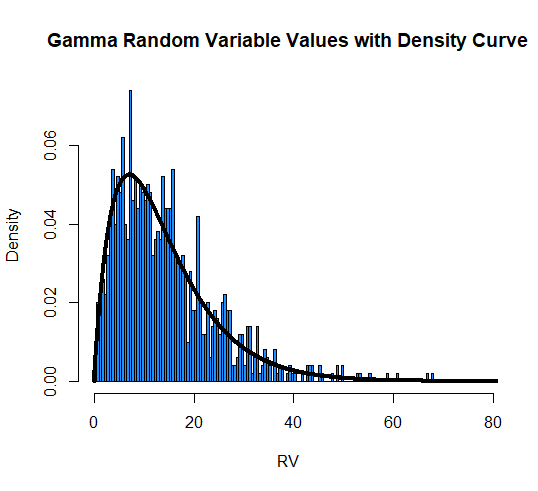
\includegraphics{week2/GammaSimOne.png}
                
            \subsection{}
                The exact proportion below 4 for the simulation was 0.11. This matches fairly closely with the expected value found in part 2.iii.\\
                
            \subsection{}
                The increasing number of trials has had the effect of a much tighter fit to the curve. There are still some values that are inside or outside the curve. However, Those values are much less extreme than the trial where we only ran one thousand trials.\\
                
                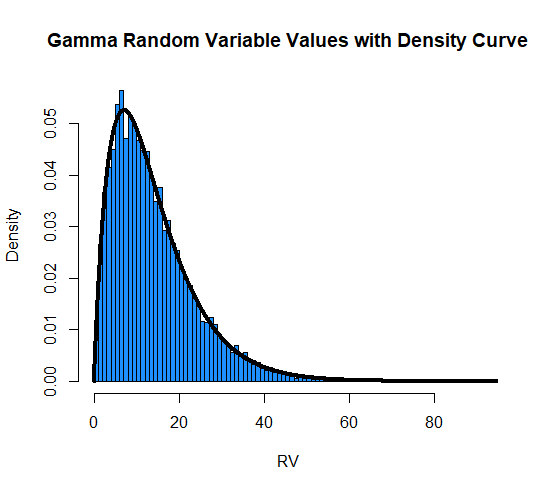
\includegraphics{week2/GammaSimTwo.png}
            \subsection{}
		        In the second trial I had 11.56 percent of the values below 4. This seems a bit high in comparison to our expected value of 11.26. Looking at the plot it seems I may have a few outliers that are throwing this off. This is about the same amount of error in the first trial with 1000 points. However, This one was off on the high side rather than the low side.\\
		        
		    \subsection{}
		        When running the gamma simulation with Alpha set to one I find that the shape of the data looks like it is exponential. The probability density starts off high and gets lower and lower over time.\\
		    
		        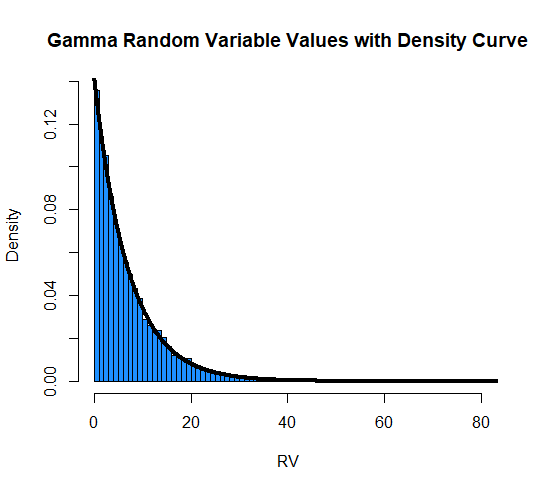
\includegraphics{week2/GammaSimThree.png}
		        
            \subsection{}
                The above simulation is the Exponential Distribution. As noted before the shape looks like it fits the exponential model. This is because the exponential distribution is the same as the Gamma distribution when alpha is one.\\
                
                Below is the expression that represents the probability density function.
                
                \[
		        f_x =
		        \begin{cases}
		            \frac{1}{7}e^{-\frac{1}{7}x} &\  x \geq 0\\
		            0 &\ x < 0\\
		        \end{cases}
		        \]\\
                
                
		        
	
		\end{document}